
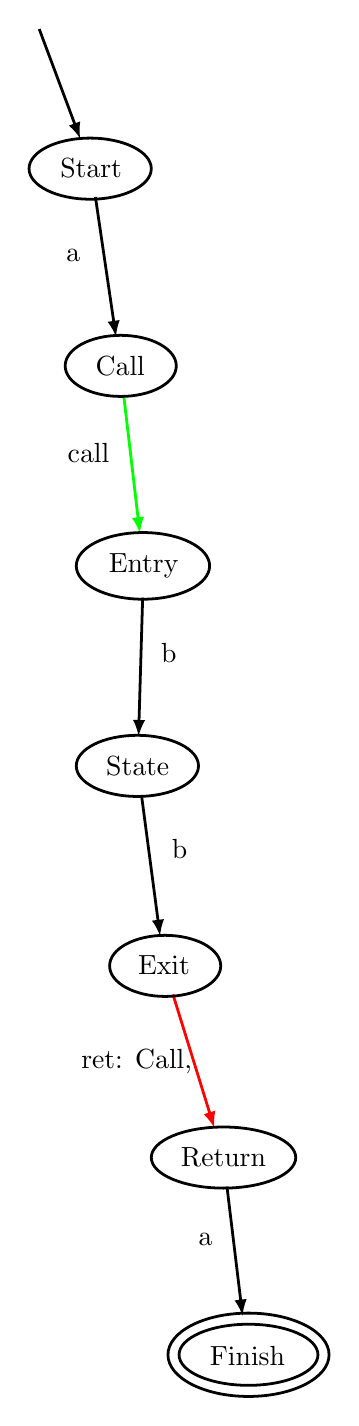
\begin{tikzpicture}[>=latex,line join=bevel,]
  \pgfsetlinewidth{1bp}
%%
\pgfsetcolor{black}
  % Edge: Call -> Entry
  \pgfsetcolor{green}
  \draw [->] (65.088bp,361.28bp) .. controls (66.298bp,350.94bp) and (68.176bp,334.88bp)  .. (70.882bp,311.74bp);
  \definecolor{strokecol}{rgb}{0.0,0.0,0.0};
  \pgfsetstrokecolor{strokecol}
  \draw (52.396bp,340.55bp) node {call};
  % Edge: Entry -> State
  \draw [->] (71.893bp,288.55bp) .. controls (71.58bp,277.93bp) and (71.109bp,261.96bp)  .. (70.424bp,238.73bp);
  \draw (81.311bp,268.81bp) node {b};
  % Edge: Start -> Call
  \draw [->] (54.89bp,432.78bp) .. controls (56.443bp,422.22bp) and (58.873bp,405.7bp)  .. (62.293bp,382.45bp);
  \draw (46.851bp,411.65bp) node {a};
  % Edge: Return -> Finish
  \draw [->] (102.24bp,76.549bp) .. controls (103.39bp,67.04bp) and (105.12bp,52.698bp)  .. (107.86bp,30.084bp);
  \draw (94.431bp,57.427bp) node {a};
  % Edge: Exit -> Return
  \pgfsetcolor{red}
  \draw [->] (82.809bp,145.71bp) .. controls (85.952bp,135.57bp) and (90.797bp,119.93bp)  .. (97.68bp,97.708bp);
  \definecolor{strokecol}{rgb}{0.0,0.0,0.0};
  \pgfsetstrokecolor{strokecol}
  \draw (69.75bp,121.53bp) node {ret: Call, };
  % Edge: State -> Exit
  \draw [->] (71.498bp,217.28bp) .. controls (72.895bp,206.7bp) and (75.081bp,190.13bp)  .. (78.158bp,166.82bp);
  \draw (85.161bp,198.1bp) node {b};
  % Edge: Start__precursor__ -> Start
  \draw [->] (34.658bp,493.26bp) .. controls (38.103bp,484.05bp) and (42.322bp,472.78bp)  .. (49.408bp,453.83bp);
  % Node: Finish
\begin{scope}
  \definecolor{strokecol}{rgb}{0.0,0.0,0.0};
  \pgfsetstrokecolor{strokecol}
  \draw (110bp,16bp) ellipse (25bp and 11bp);
  \draw (110bp,16bp) ellipse (29bp and 15bp);
  \draw (109.62bp,15.5bp) node {Finish};
\end{scope}
  % Node: Return
\begin{scope}
  \definecolor{strokecol}{rgb}{0.0,0.0,0.0};
  \pgfsetstrokecolor{strokecol}
  \draw (101bp,87bp) ellipse (26bp and 11bp);
  \draw (100.96bp,87.117bp) node {Return};
\end{scope}
  % Node: Exit
\begin{scope}
  \definecolor{strokecol}{rgb}{0.0,0.0,0.0};
  \pgfsetstrokecolor{strokecol}
  \draw (80bp,156bp) ellipse (20bp and 11bp);
  \draw (79.559bp,156.2bp) node {Exit};
\end{scope}
  % Node: Start
\begin{scope}
  \definecolor{strokecol}{rgb}{0.0,0.0,0.0};
  \pgfsetstrokecolor{strokecol}
  \draw (53bp,443bp) ellipse (22bp and 11bp);
  \draw (53.339bp,443.33bp) node {Start};
\end{scope}
  % Node: State
\begin{scope}
  \definecolor{strokecol}{rgb}{0.0,0.0,0.0};
  \pgfsetstrokecolor{strokecol}
  \draw (70bp,228bp) ellipse (22bp and 11bp);
  \draw (70.103bp,227.85bp) node {State};
\end{scope}
  % Node: Call
\begin{scope}
  \definecolor{strokecol}{rgb}{0.0,0.0,0.0};
  \pgfsetstrokecolor{strokecol}
  \draw (64bp,372bp) ellipse (20bp and 11bp);
  \draw (63.851bp,371.86bp) node {Call};
\end{scope}
  % Node: Entry
\begin{scope}
  \definecolor{strokecol}{rgb}{0.0,0.0,0.0};
  \pgfsetstrokecolor{strokecol}
  \draw (72bp,300bp) ellipse (24bp and 12bp);
  \draw (72.236bp,300.17bp) node {Entry};
\end{scope}
%
\end{tikzpicture}
